\documentclass[12pt]{article}

\usepackage{graphics}
\usepackage{epsfig}
\usepackage{times}
\usepackage{amsmath}

% <http://psl.cs.columbia.edu/phdczar/proposal.html>:
%
% The standard departmental thesis proposal format is the following:
%        30 pages
%        12 point type
%        1 inch margins all around = 6.5   inch column
%        (Total:  30 * 6.5   = 195 page-inches)
%
% For letter-size paper: 8.5 in x 11 in
% Latex Origin is 1''/1'', so measurements are relative to this.

\topmargin      0.0in
\headheight     0.0in
\headsep        0.0in
\oddsidemargin  0.0in
\evensidemargin 0.0in
\textheight     9.0in
\textwidth      6.5in

\title{{\bf Doctoral Thesis Proposal} \\
\it Thesis proposal}
\author{ {\bf Kangkook Jee}  \\
Department of Computer Science \\
Columbia University\\
{\small jikk@cs.columbia.edu}
}
\date{\today}

\begin{document}
\pagestyle{plain}
\pagenumbering{roman}
\maketitle

\pagebreak
% !TEX root = proposal.tex
\begin{abstract}

%While our everyday dependency to the computer-based services gets more and more
%significant, it is becoming more difficult to protect it from attackers
%motivated for increased revenue, and equipped with wide range of attack vectors
%for their malicious activities.

%
A common way to harden software systems against failures due to malicious
attempts from attackers or unexpected disclosure of developer bugs, is to
in-line security and monitoring logics to be executed simultaneously.
%
Being effective in defending against these failures, the approaches based on
in-line monitors have suffered from inherent issue of too high overhead which
subsequently hinders the approach's production system adoptation.

Addressing the issue, a number of proposals for parallel execution arose from
the past proposals,
%that decouples two different contexts~(the one for the original execution and
%the other for monitoring logics) and let each run from different CPU cores
%arose from the past proposals, 
but most of them have failed to be a practical solution most notably for having
too high communication cost between two threads(contexts).
%
%Addressing the issue, I implemented a framework that parallelize  Data flow
%Tracking~(DFT) minimizing the amount of communcation required between the
%original and analysis thread.

From this document, I want to propose a methodology that defines the optimal
amount of information needed from the original execution required to restore
the correct monitoring context from another thread.
%
One intermediate result, I presented a system that parallelize DFT analysis,
which implements the methodology from offline static analysis which in turn
could achieve x2.75 slowdown over native execution when it is evaluated for
SPEC 2006 CPU benchmarks.
%
Generalizing the approach, I am planning to advance the research direction to
see how can we apply the approach so that dfferent type of ananalyses by
defining a guide and anc common API. 
%
As a next step, we will explore design choices available for
instrumentation/in-lining layer required for event collection and communcation.
This direction of research will i) improve VM-based instrumentation
which is currently employed ii) propose H/W component to support
parallelized analysis in broad/general sense.


%%
%While our everyday dependency to the computer-based services gets more and more
%significant, it is becoming more difficult to protect it from attackers
%motivated for increased revenue, and equipped with wide range of attack vectors
%for their malicious activities.
%%
%Number of different security systems have been proposed to defend software
%systems against such threats, but none has succeeded yet for a number of
%reasons. 
%% effectiveness issue
%Firstly, some security measures are not capable of protecting softwares against
%certain attack methods or being accurate in defining malicious activities.
%% efficiency issue
%Secondly, some other measures can counter most of attack vectors with
%reasonable accuracy but it incurs non-negligible amount of overhead and
%prevents wide adaptation. 
%
%In my past efforts to build a security system that address the aforementioned
%issues, I developed and improved a security system of DFT by leveraging
%VM-based instrumentation to in-line its monitoring logics. 
%%
%Even with the substantial amount of performance improvement my work could make
%for DFT system, I should admit that it has not yet reached to the point where
%industry and research community would consider it as adoptable to their
%production systems.
%
%In this document, I propose a number of research directions that would address
%aforementioned issues.
%%
%% by exploring various design choice from different layers of computer systems
%% and establishing a measurement framework that evaluates the accuracy of the
%% security system.
%%
%Our past innovations for DFT can be further enhanced leveraging opportunities
%available from different layers of the computer system. I will also verify that
%we can build an evaluation framework that would systematically infer invariants
%regarding correctness of DFT operations.
%%
%% filling gap between semantic understanding and instruction level
%% implementations.
%%
%Lastly, I will confirm that these experience can be generalized and extended to
%implement different security measures.
%%


\end{abstract}


\pagebreak
\tableofcontents
\pagebreak
% !TEX root = proposal.tex
\section{Introduction} 
\label{sec:intro}

Protecting software system is a challenging task. 
%
Attack vectors available to attackers are often unknown and this leads to
incapable of defending zero day attacks.
%
Developers make mistakes in their codes.

% Securing/positioning the document -- needs elaboration.
%
In respond to these problems, we have seen many proposals that
inject/instrument one or more type of monitoring logics~\cite{cfi, memcheck,
dft} against the program that we want to protect and let them run
simultaneously to defend against various types of unexpected behaviors.
%
Research has been exploring three different approaches to instrument/in-line
monitoring logics to implement in-line monitors.
%
Number of criteria to compare and evaluate different approaches. efficiency,
coverage, flexibility(general ?).

\begin{itemize}
%
    \item {\bf Source code based:} Leveraging different representations exposed
in the process of program build. Abstract Syntax Tree~(AST) or compiler
specific Intermediate Representations~(IR) can be an instrumentation target.
This approach is reasonably fast incurring about or less than $\sim$ 2$\times$
overhead, but it can encounter an issue related to code {\it coverage} as in
most case we only have a partial source access about program's execution
environment for having 3rd party libraries~(\ie libc) that come as binaries.
%
    \item {\bf Hardware assisted:} This approach leverages hardware add-ons to
instrument monitoring defense logics to a runtime execution and it is the most
efficient approach being able to achieve near-to-native performance. The
approach is not flexible as users cannot modify monitoring logics once it is
fixed/burned/encoded to hardware. This is also not general as we have not seen
any commodity vendors that implements this kind of in-line monitors.
%
    \item {\bf VM-based instrumentation:}  This approach leverages widely
adopted VM-hypervisor for instrumentation. As this approach overcomes the
coverage issue supporting unknown(COTS) binaries and users can freely modify
and update their monitoring logics, the approach incurs to much runtime
overhead.

\end{itemize}
%
The approach based on VM-based instrumentation, being effective in defending
software systems against aforementioned threats, is regarded as the most
promising for its ability to address limitation of other approaches -- coverage
and flexibility. 
%
However the approach suffers from excessive amount of slowdown and the sources
for the overhead are {\it i)} instrumentation cost needed to maintain two
different contexts {\it ii)} cycles for defense/monitoring logic itself.
%

The idea of parallel analysis that decouples the original application and
analysis logics and executes these contexts from different execution
units~(threads) has risen from past research to minimize the runtime overhead.  
%
We have two different approaches based on process replication and subset state
propagation.
%
The cost for the communication connecting two threads tends to be too
high/excessive for both approaches, subsequently masks/overwhelms/cancels the
parallelization benefit and often make it slower than comparable in-lined
analysis. Its side-effects include

\begin{itemize} \item n analyzer threads.  \item synchronization becomes too
difficult.  \item not suitable for online/runtime analysis. In turn, some are
purely positioned themselves as an off-line solution.  \end{itemize}

%Preliminary result -- explain ShadowReplica, TFA, libdft
From my previous research~\cite{ShadowReplica, TFA}, I proposed a system that
directly addresses the issue of too high communication overhead for an analysis
of Data Flow Tracking~(DFT). The system identifies minimal but necessary
elements from the original executions and then establishes a framework that
applies number of optimizations to properly compress the runtime communication
which eventually contributes to {\it i)} minimize the mitigation of event
collection to the original execution, {\it ii)} minimize the communication
traffic, and {\it iii)} make the analysis thread run faster than the original
thread.

%what this proposal is about.
From this document, I propose an approach that generalizes my previous work
that defines the minimal amount of information required from arbitrary program
execution applicable to restore wider range of in-lined monitors from another
threads.
%
For this, I provide framework for to categorize available in-line
monitors~\cite{CAB} with number of abstractions for necessary/implemented
functionalities common to these analyses which, I expect, would help us to
define common API exposed to users to implement their own parallelized
analysis.
%
Then, I investigate the general and specific optimizations applicable to each
analyses.


% !TEX root = proposal.tex
\section{Background and Related Work}
\label{sec:related}

In this section, I discuss related work and present my previous research
results relevant to my thesis to help reader to identify the context of this
thesis proposal.

\subsection{Related Work}

\subsubsection{Inline Monitors}
\label{ssec:inline}

Program protection and profiling using inline monitors are dynamic analysis
approaches that execute specific analysis logics along with the application
process. Instance of the technology includes data flow tracking
(DFT)~\cite{DFT}, memory integrity checking~\cite{memcheck}, control flow
integrity~\cite{cfi}, method counting, call graph profiling and so on.
Given that the technology can be implemented interleaving analysis/monitoring
logics into the program execution, we can choose different instrumentation
targets either of source code or program binaries and use different
instrumentation mediums to implement inline monitors.

Employing source code based approach, we can use representations
exposed~\cite{AST,LLVM-IR} by compiler internals as instrumentation targets or
source-to-source approaches~\cite{txl, cil} to make changes to source code.
This approach comes in reasonable amount of overhead roughly around $2\times$
or less, but it is limited in completeness not being able to support COTS
binaries (\ie 3rd party libraries).  An alternative can be binary
implementation approaches either based on process-wide virtualization using
dynamic binary instrumentation(DBI)~\cite{PIN, dynamoRIO, valgrind} or
system-wide virtualization~\cite{qemu,xen}. These address coverage issue as
these can handle unknown program binaries. However, it comes with excessive
amount of overhead which vary from $\times 5 \sim \times 100$ based on analyses
and application domains. Hardware assisted implementation~\cite{HARD, lba} can
implement inline monitors with minimal amount of overhead less than 5\% at most
supporting full coverage, but the we have not yet seen this functionality
supported by major vendors with their commodity production.

\subsubsection{Data Flow Tracking (DFT)}

DFT is one of inline monitoring approaches that accurately tracks selected data
of interest, as they flow during program execution. Among other uses, DFT has
been employed to provide insight in the behavior of applications and systems,
and to assist in the identification of configuration errors. Most prominently,
it has been used in the security field to defend against various software
exploits~\cite{}, and to enforce information flow by monitoring and restricting
the use of sensitive data~\cite{}. For the former, the network is usually
defined as the source of interesting or “tainted” data, while the use of
tainted data is disallowed in certain program locations (\eg, in instructions
manipulating the control flow of programs, such as indirect branch instructions
and function calls). For the latter, the developer or the user is responsible
for specifying the data that needs to be tracked and the restrictions on their
use. DFT is even used to assist solving performance problems~\cite{} pairing
configuration file entries with performance bottlenecks as sources and sinks. 

DFT is implemented by having shadow context that corresponds to the original
execution context. The shadow context comprise of shadow operations and shadow
memory area. Table~\ref{tab:dft_tracking} shows how instructions' DFT semantics
for general purpose instruction architecture (ISA) are defined to perform DFT
operations to keep track of changes from shadow memory area. 

\begin{table}[h]
        \centering
\begin{tabular}{|l|l|}
\hline
{\bf Instruction} & {\bf Tag propagation rule} \\ \hline \hline
    {\tt \specialcell{ALU-OP OP1 $\leftarrow$ OP2 \\ (add, sub \dots)}} & 
    {\tt t(op1) $\vert=$ t(op2)}\\ \hline
    {\tt MOV OP1  $\leftarrow$  OP2} & {\tt t(op1) = t(op2)}     \\ \hline
    {\tt LOAD OP1 $\leftarrow$ [OP2]} & {\tt t(OP1) = t([OP2])}  \\ \hline
    {\tt STORE [OP1] $\leftarrow$ OP2} & {\tt t([OP1]) = t(OP2)} \\ \hline
\end{tabular}
\caption{presents an interpretation of DFT semantics for pseudo instruction set
architecture.}
\label{tab:dft_tracking}
\end{table}

The specifics of DFT can vary significantly depending on ones goals,
performance considerations, and deployment platform. One possible
classification of existing mechanisms can be made based on the means by which
the tracking logic is augmented on regular program execution. As we discussed
from Section~\ref{ssec:inline}, DFT can be performed by inserting data tracking
logic statically during the compilation of software, or by performing source-
to-source code transformation~\cite{}. It can also be applied dynamically by
augmenting instrumentation code on existing binaries using dynamic binary
instrumentation (DBI)~\cite{}  or a modified virtual machine (VM)~\cite{}.
Finally, DFT can be also performed in hardware~\cite{}.

\subsubsection{Parallelized Analysis}
\label{ssec:parallel}

The idea of decoupling dynamic program analyses from execution, to run them in
parallel, has been studied in past in various contexts~\cite{} . 
%
Aftersight~\cite{}, ReEmu~\cite{}, and Paranoid Android~\cite{} leverage record
and replay for recording execution and replaying it, along with the analysis,
on a remote host or a different CPU (replica). They are mostly geared toward
off-line analyses and can greatly reduce the overhead imposed on the
application.  However, the speed of the analysis itself is not improved, since
execution needs to be replayed and augmented with the analysis code on the
replica.  SuperPin~\cite{} and Speck~\cite{} use speculative execution to run
application and (in-lined) analysis code in multiple threads that execute in
parallel. These systems sacrifice significant processing power to achieve speed
up.  Furthermore, handling multi-threaded applications without hardware support
remains a challenging issue for this approach. CAB~\cite{} and PiPA~\cite{} aim
at offloading the analysis code alone to another execution thread, and they are
the closed to \sreplica. However, neither of the two has been able to deliver
the expected performance gains, due to {\it (i)} naively collecting information
from the application, and {\it (ii)} the high overhead of communicating it to
the analysis thread(s). 

\subsection{Previous Research}

From my previous research, I have addressed the high overhead issue inherent to
heavy-weighted inline monitors such as DFT implementations.

\subsubsection{\libdft}

\libdft is a highly optimized DFT framework that shows comparable to or faster
performance than most previous DFT implementations. \libdft implements
instruction level monitors by instrumenting DFT instruction that perform shadow
operations against {\tt x86} binary stream at runtime using PIN~\cite{} DBI
framework.
%
\libdft's performance gain comes in two folds. 

The first optimization is by having {\it inline-friendly} DFT operations. To
interleave codes from two different contexts, underlying DBI framework should
add management instructions to save and restore states relevant to each context
for every instrumentation. The state includes the whole CPU registers and the
operation of spilling/re-filling these is typically expensive. {\it
Instrumentation inlining}~\cite{} reduces this overhead taking advantage of
remaining register entries unused from the application context. In order to
make DFT operations to be instrumentation suitable for inlining, it needs to
meet the following two conditions.
%
\begin{enumerate} \item The instruction count for DFT operation should less
than ten.  \item DFT operation should not contain branch operations that make
updates to {\tt EFLAG} register.  \end{enumerate} 
%
Having highly crafted routines that satisfy above conditions, \libdft could
have most of its operations in-lined reducing signification amount of overhead.

The second optimization is by having optimal shadow memory design that
minimizes the cycles needed to translate real address entries into shadow
memory counterparts. We have number of design choices regarding shadow store
structure that come with CPU time vs. memory space trade-offs. Not to reduce
the execution transparency by assign too large portion of address space, most
of shadow memory architectures leverage multiple level of indirections which
inevitably involve conditional operations. \libdft avoids this problem by
instrumentation every memory routines to co-allocate/deallocate counterpart
shadow entries. This not only reduce the instruction counts but also eliminate
need for control instruction in translations.

\libdft takes the form of a shared library enabling developers to create of
DFT-enabled Pintools for binaries, using its extensive API. For example,
\libdft already includes a DTA tool, which can be used to protect applications
from remote buffer overflow exploits.

\subsubsection{\tfa} 

Main insights behind \tfa is that update-to-date DFT are lacking in {\it i)}
consideration for global context {\it ii)} understanding of DFT operation
semantics which is different from the original execution semantics.  \tfa
attempts to address these issues by dedicating off-line static phase that
performs application and DFT specific analysis. 

\begin{figure}[tb]
    \centering
%        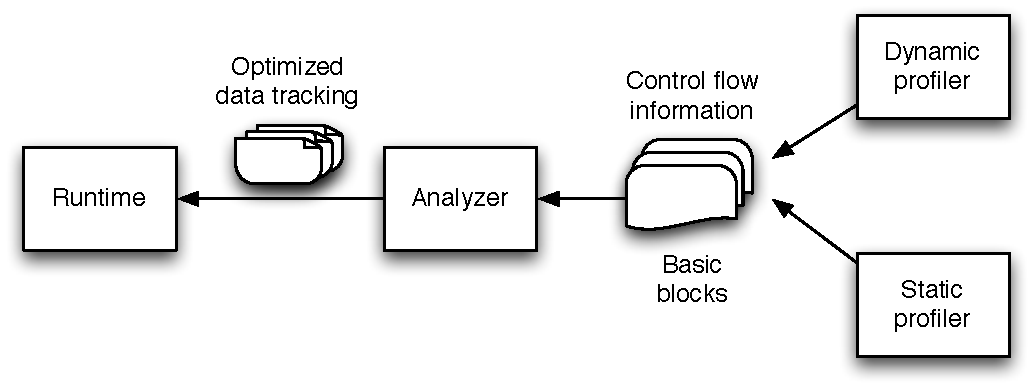
\includegraphics[width=\linewidth]{figs/execution_model.pdf}
    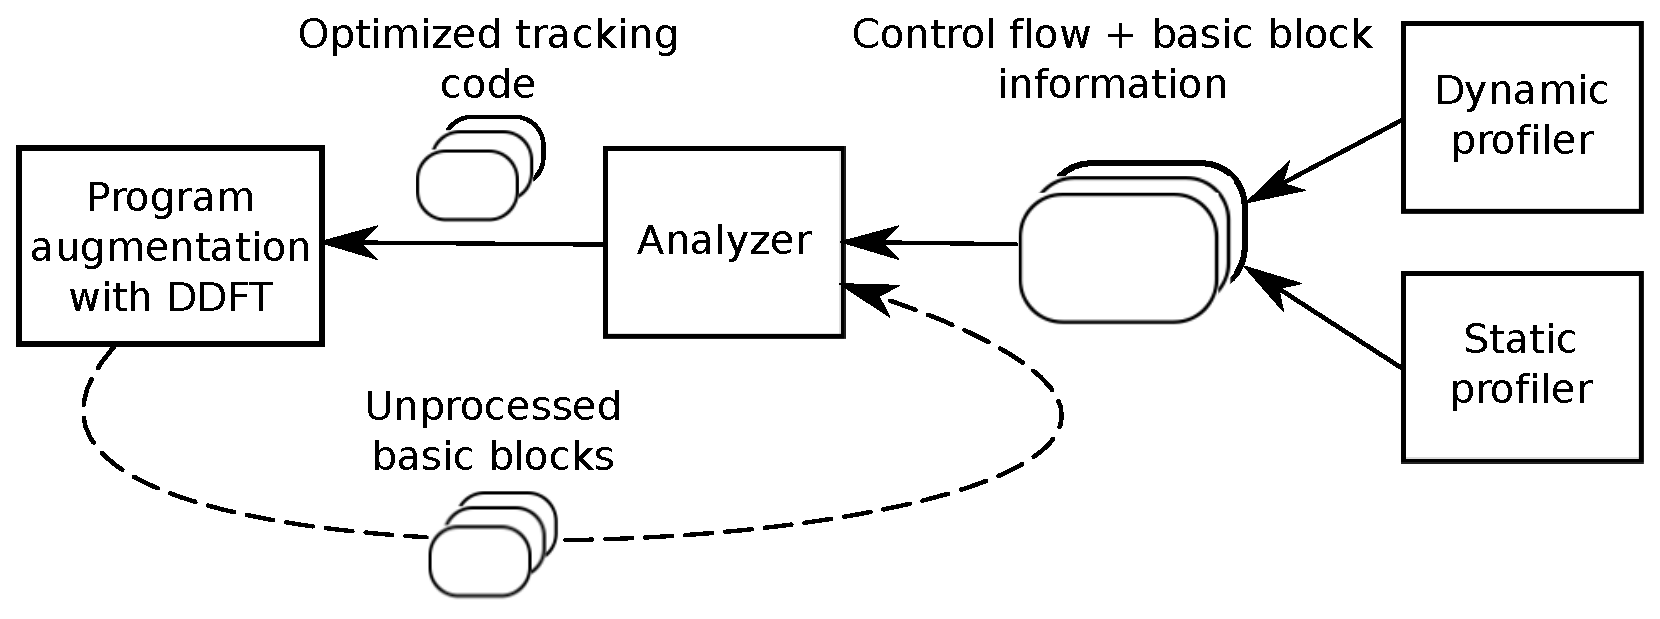
\includegraphics[width=0.6\linewidth]{figs/overview_model.eps}
    \caption{\tfa overview: It extract basic blocks and control flow
    information using a combination of dynamic and static analysis, and then
    statically analyze this information to produce optimized data tracking
    code.
   \label{fig:approach_overview}}
\end{figure}

Figure~\ref{fig:approach_overview} shows a high-level overview of our approach
for optimizing data tracking. We start by dynamically and statically profiling
the target application to extract its basic blocks and control flow
information. A basic block (BBL) of code consists of a sequence of instructions
that has only one entry point and, in our case, a single exit point. This means
that no instruction within a BBL is the target of a jump or branch instruction,
and the block is only exited after its last instruction executes. These
properties are desirable for various types of analysis, like the ones performed
by compilers. The control flow information describes how the basic blocks are
linked. The combination of dynamic and static profiling provides us with a
significant part of the CFG, including the part that dominates in terms of
execution time, and would benefit the most from optimization.
%
The analyzer receives the profiler information and extracts data dependencies
from the code, separating program from data tracking logic. It then transforms
the latter to an internal representation, based on the Taint Flow Algebra
(\tfa), which is highly amenable to various optimizations. The optimizations
performed by the analyzer and include classic compiler optimizations like
dead-code elimination and copy propagation as well as DFT specific ones. Our
goal is to remove redundant tracking operations, and reduce the number of
locations where tracking code is inserted. 
%
Finally, the analyzer emits optimized tracking code, which is applied on the
application. Note that the type of tracking code generated depends on the
original tracking implementation to be optimized. Implementation, as it
operates on binary programs the analyzer produces primitive C code, which can
be compiled and inserted into the application using a DBI framework.

\tfa extends \libdft re-using many features such as instruction interpretation
and shadow memory design. More importantly, \libdft plays a role of slow-path
DFT implementation to cover execution paths missed from static analysis phase
ensuring the completeness of our approach.
 
\subsubsection{\sreplica}



\cleardoublepage
\pagenumbering{arabic}

\pagebreak

\begin{footnotesize}
\bibliographystyle{plain}
\bibliography{string,itu,rfc,i-d}
\end{footnotesize}

\end{document}


